\chapter{Platinenentwurf}\label{kap5}
Im Folgenden wird die Gedankengänge und Einflüsse eingegangen, die zum endgültigen Platinendesign geführt haben, eingegangen. Dabei wird neben der reinen Platinenbetrachtung auch die Rahmenbedingungen erläutert.
\section{Elektronikgehäuse und Anforderungen an die Platinendimensionierung}
Die Platine wird in ein Gehäuse eingebettet, welches parallel zu und in Absprache mit dieser Arbeit entwickelt wurde. Die Anforderung, den Aktor durch die entwickelte Elektronik zu einem \textit{Smart Actuator} zu transformieren wird erfüllt, in
dem die Platine durch das Gehäuse am Aktorgehäuse verschraubt wird. \autoref{fig:gh1} zeigt schematisch die Lage der Platine (grün) im Gehäuse. In grau ist der Verbindungsstecker zu sehen, der abgedichtet im Gehäuse liegt. Anschließend wird ein Deckel montiert, wodurch die Elektronik von Schmutzpartikeln und anderen Umwelteinflüssen geschützt wird. Dieser ist aus Übersichtsgründen nicht abgebildet.

\begin{figure}[H]%
\centering
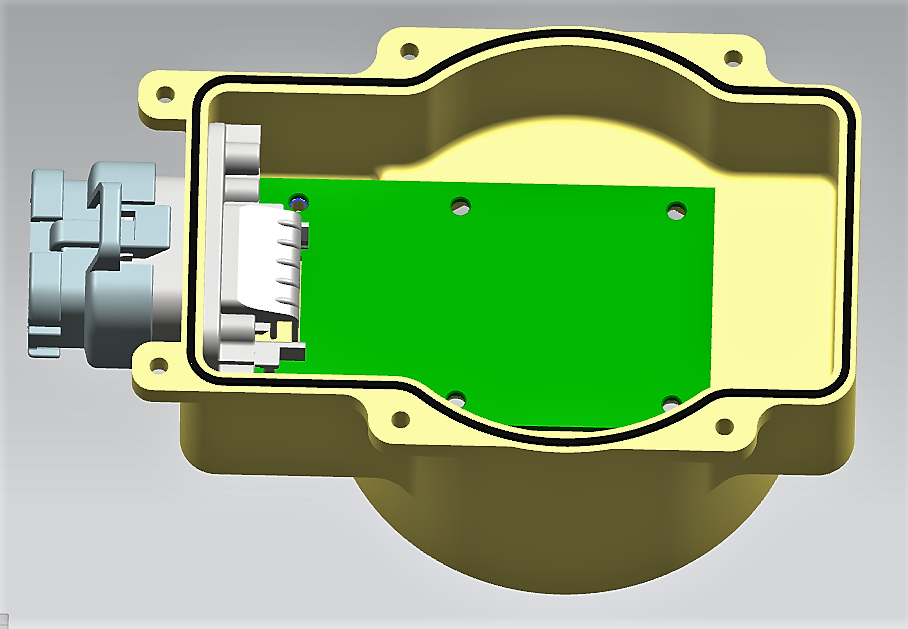
\includegraphics[width=300pt]{./Bilder/Elektronik_Gehauese_ver3}%
\caption{Derzeitiger Entwurf des Elektronikgehäuses}%
\label{fig:gh1}%
\end{figure}

Durch die Größe des Aktors ergeben sich Höchstmaße an das Platinengehäuse und die Platine selbst. Um ein Einbauen zu garantieren, dürfen die Außenmaße der Platine $\SI{88,8}{mm} \cdot \SI{50}{mm}$ nicht überschreiten. In diesem Fall war der Platz ausreichend, um alle nötigen Schaltungen und Funktionen auf der Platine zu verwirklichen. Als Ausweichlösung, falls die ebenen Maße nicht ausgereicht hätten war angedacht, die Elektronik auf zwei Platinen aufzuteilen (z.B. Logik- und Leistungsteil), und sie in zwei Ebenen parallel übereinander anzuordnen. Dies ist weiterhin denkbar, falls die Elektronik erweitert werden soll. Gelötete Teile auf der Platine, welche einen großen Bauraum nach oben benötigen sind vor allem der THT Kondensator mit \SI{1000}{\mu F} sowie die Wire-to-Board Reihenklemmen. Diese sind bereits auf der linken Seite (Steckerseite) der Platine angeordnet, sodass über der rechten Seite relativ unproblematisch eine zweite Platinenebene eingeführt werden könnte.
Da das Gehäuse aufgrund von kostengünstiger und einfacher Fertigung aus Kunststoff geplant und hergestellt wurde, muss eine Lösung gefunden werden um die Platine mit GND zu verbinden, zu kühlen und elektromagnetisch abzuschirmen. Es bietet sich an, eine Aluminiumplatte, die den Maßen der Platine entspricht, zwischen Platine und Gehäuse anzubringen. Dabei wird auf Aluminium zurückgegriffen, da es sich um ein kostengünstiges, leitfähiges Metall handelt, welches außerdem eine hohe Wärmeleitfähigkeit von \SI{204}{\frac{W}{mK}} besitzt \cite[S.4]{wuerth}. 
Durch das Loch in der Unterseite des Gehäuses, welches in \autoref{fig:gh2} zu erkennen ist, liegt die Aluminiumplatte, in dieser Darstellung grün eingefärbt, am Aktorgehäuse an. Das hat den Vorteil, dass die Platine Wärme an die Aluminiumplatte über Konduktion abgeben kann, welche wiederum ihre Wärme an das Aktorgehäuse aus Aluminium abgibt. Diese Wärmeübertragung soll durch Wärmeleitpaste beziehungsweise –kleber unterstützt werden. Diese Lösung erspart weitere externe Kühlkörper. Diese Methode hat die Einschränkung, dass nur die aluminiumfreie Seite der Platine bestückt werden darf, ansonsten müssen die betroffenen Bereiche in der Aluminiumplatte ausgespart werden. Da die Platine mit THT-Bauteilen teils auch auf der Unterseite verlötet werden musste, wurden die nötigen Aussparungen durch Bohrlöcher realisiert. 
\begin{figure}[H]%
\centering
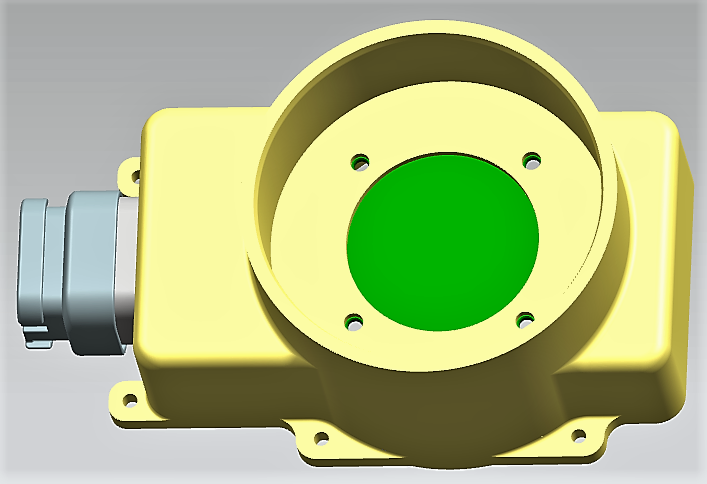
\includegraphics[width=300pt]{./Bilder/Elektronik_Gehauese}%
\caption{Rückseite des Elektronikgehäuses zur Darstellung der Aktoranbindung}%
\label{fig:gh2}%
\end{figure}
Die vier Schrauben, mit denen Platine, Aluminiumplatte und Platinengehäuse am Aktorgehäuse verschraubt werden, sorgen zusätzlich für einen optimalen Wärmeübergang von Platine bis zum Aktor. Diese vier Schraubverbindungen plus zwei weitere Schraubverbindungen, welche Platine, Aluminiumplatte und Platinengehäuse verbinden, ermöglichen außerdem eine großflächige GND-Verbindung über die Aluminiumplatte. Die Auflageflächen der Schrauben sind jeweils auf GND-Potential gesetzt, sodass Schrauben und Platte auch dieses Potential annehmen.
Eine weiterer wichtiger Aspekt den es bei Platinengehäusen zu beachten gilt, ist die notwendige Abschirmung gegen Eintreten sowie Abstrahlung elektromagnetischer Strahlung. Das Kunststoffgehäuse ist dabei weniger geeignet als die Aluminiumplatte, die aufgrund der elektrischen Leitfähigkeit eine gute Basisschirmung besitzt \cite{bopla}. Für Kunststoffgehäuse wird im Allgemeinen eine Beschichtung aus Aluminium oder Kupfer empfohlen \cite{Gwinner2006}.

\section{Komponentenplatzierung auf der Platine}\label{sec:bau}
Beim Layout-Entwurf müssen mehrere Aspekte berücksichtigt werden: Die Platinenmaße und die Platzierung der GND-Schrauben müssen eingehalten werden und die Lokalität der Bauteile sollte gut durchdacht sein. Beispielsweise sollten die Halbbrücken nahe an der Spannungsversorgung platziert werden, um lange leistungsführende Leitungen zu verhindern. Weiterhin müssen die Leitungen der sensiblen Sensorik gegen elektromagnetische Rückwirkung geschützt werden. Beim engültigen Platinenentwurf, welcher in \autoref{fig:docu} zu sehen ist, ist die Lokalität der Leistungs-Bauteile, also der Halbbrücken mit den Bezeichnungen HB\_1 und HB\_2, deutlich von der Platzierung der Logikebene getrennt \cite[S.26]{emcdes}. Die Halbbrücken befinden sich auf der rechten Hälfte der Platine, nahe des Steckers, wodurch lange Leistungsleitungen vermieden werden können. Der Klemmblock (\textit{terminal block}) als Anschlussklemme für den Tauchspulenaktor ist ebenfalls nahe der Halbbrückenausgänge platziert, sodass auch die Ausgangsleitungen geringe Leitungslängen aufweisen. In \autoref{fig:docu} ist dieser Block mit der Bezeichnung TB\_1 gekennzeichnet. Der Kondensator zum Stabilisieren der Batteriespannung ist als C13 gekennzeichnet und ebenfalls nahe der Spannungsversorgung platziert. Aus Platzgründen mussten auch die Klemmblöcke für Temperatur- und externe Strommessung (J2 und J3) auf der rechten Platinenhälfte platziert werden. Da sich die leistungsführenden Leitungen jedoch auf die Mitte der Platine konzentrieren stellt dies kein Problem dar. In der linken Platinenhälfte befindet sich der Logikteil, welche den Mikrocontroller (\textit{STM32}), den CAN-Transciever (CAN\_T), den externen Taktgeber (QUARZ) und den Leitungsverstärker (\textit{CD74HCT}) umfasst. Neben diesen Bauteilen befindet sich ebenfalls die Spannungsregler für \SI{3,3}{V} und \SI{5}{V}, sodass bei der Spannungsversorgung für die ICs keine Probleme durch elektromagnetische Rückwirkungen auftreten und die Versorgungsleitungen zu den Bauteilen kurz gehalten werden kann. Bei der Platzierung der Bauteile spielt ebenfalls die Ausrichtung des Mikrocontrollers eine wichtige Rolle, sodass die benötigten Pins des Mikrocontrollers möglichst geringe Entfernungen zum jeweiligen Bauteil aufweisen. Dadurch kann ein Kreuzen der Signalleitungen vermieden und die Länge reduziert werden \cite[S.17]{emcdes}. So befinden sich beispielsweise die Ausgangspins CAN1\_RX und CAN1\_TX des Mikrocontrollers in \autoref{fig:docu} auf der oberen Seite des STM32 und die Leitungen zum CAN-Transciever (CAN\_T) können deshalb leicht verlegt werden. Die Leitungen für die H-Brücke sind auf der rechten Seite des Mikrocontrollers platziert, sodass sich diese leicht zum Leitungstreiber (CD74HCT) legen lassen. Die Pins für den externen Quarz befinden sich an der unteren Seite des STM32 und somit nahe des Schwingquarzes. Gerade bei diesem Bauteil ist die Entfernung zum Mikrocontroller möglichst gering zu halten und eventuelle Leitungskapazitäten zu verhindern \cite[S.31]{stmquarz}. Ebenfalls sollte der Taktgeber möglichst weit von den Halbbrücken entfernt platziert sein um Störungen durch Hochfrequenzsignalen vorzubeugen \cite[S.31]{stmquarz}.
Die Entkopplungskondensatoren der ICs sollten möglichst nahe an den Versorgungseingängen platziert werden, sodass beispielsweise die Entkopplungkondensatoren C10 und C11 nahe des VDD Pins des Mikrocontrollers (STM32) liegen \cite[S.17]{emcdes}.

\begin{figure}[H]%
\centering
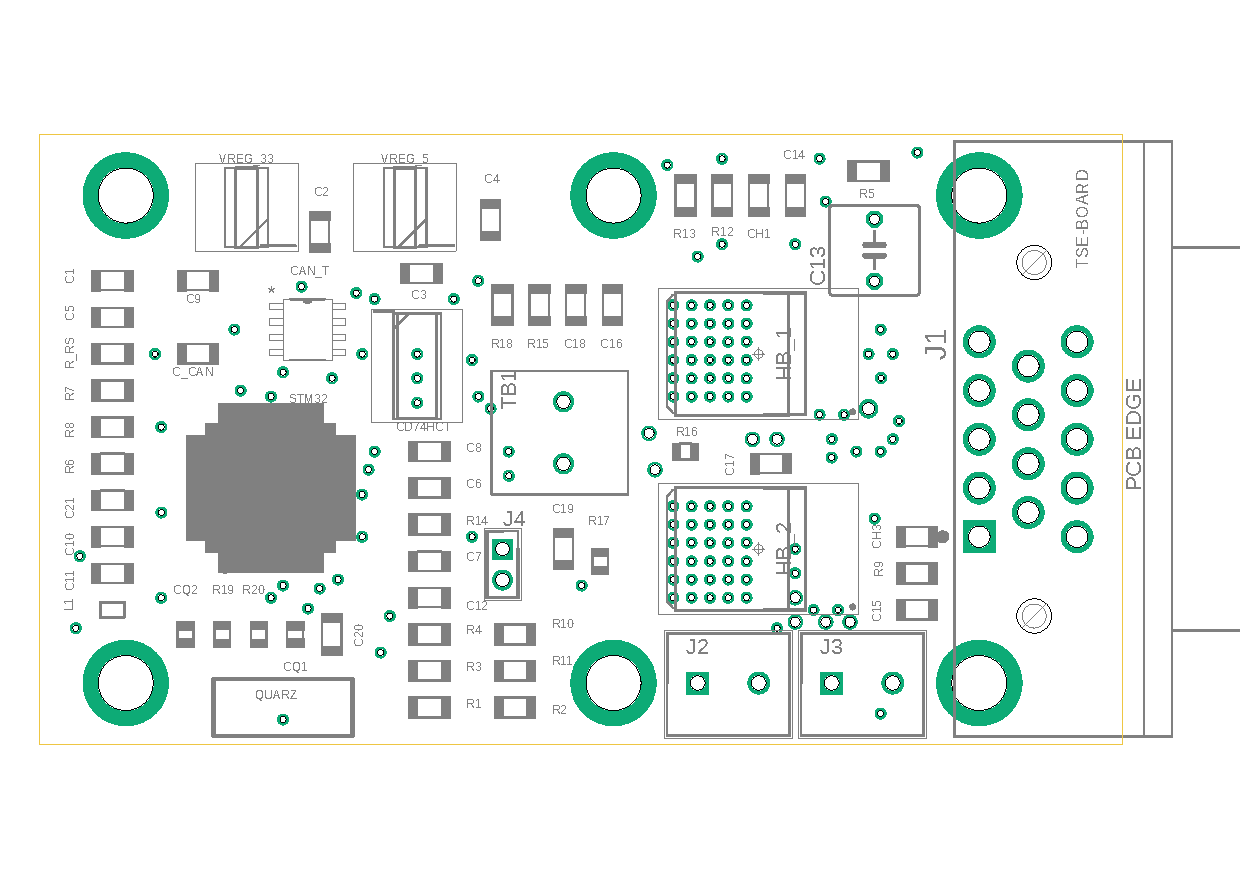
\includegraphics[width=380pt]{./Bilder/docu}%
\caption{Platzierungsgrafik der Bauteile}%
\label{fig:docu}%
\end{figure}

\section{Dimensionierung der Leiterbahnen}
Um die Leiterbahnbreite für die Halbbrücken berechnen zu können, müssen die besonderen Gegebenheiten eines Schaltvorgangs beachtet werden. Es handelt sich um Kurzzeitbelastungen im zeitlichen Rahmen von maximal \SI{100}{ms} mit einer Stromstärke von maximal \SI{60}{A}. Aufgrund der Kurzzeitbelastung können die Leitungsquerschnitte deutlich geringer gewählt werden, als die Strombelastbarkeit nach der Norm IPC 2221 es für Leiterbahnen unter Dauerlast zulässt.\\
In einem stromdurchflossenen elektrischen Leiter entsteht Verlustleistung gemäß
\begin{align*}
P = I^{2}R
\end{align*}
da Energie aufgrund des Leitungswiderstandes 
\begin{align*}
R = \rho \frac{l}{A}(1+\alpha_{r}(T(t)-T_{r})
\end{align*}
dissipiert. Dieser Leitungswiderstand hängt sowohl von den materialabhängigen Konstanten $\rho$ (spezifischer Widerstand) und $\alpha_{r}$ (Temperaturkoeffizient zur Referenztemperatur $T_{r}$), als auch von der Leiterlänge $l$, dem Leiterquerschnitt $A$ und der Temperaturänderung $T(t)$ zur Referenztemperatur $T_{r}$ ab. Aufgrund der Erwärmung der Leiterbahn durch die Verlustleistung ist die Temperaturänderung zeitabhängig. Nach dem Stromwärmegesetz gilt für die Ableitung der Wärmeenergie nach der Zeit
\begin{align}
\label{eq:dif2}
\frac{\partial Q_{W}}{\partial t} = P = I^{2}\rho \frac{l}{A}(1+\alpha_{r}(T(t)-T_{r}).
\end{align}
Die Änderung der Wärmeenergie führt zu einer Änderung der Temperatur welche sich mittels Wärmekapazität $C$ beschreiben lässt
\begin{equation}
\label{eq:waermeaend}
 Q_{W} = (T(t)-T_{r})C_W,
\end{equation}
wobei sich die Wärmekapazität aus dem Produkt der materialabhängigen spezifischen Wärmekapazität $c$ und der Masse $m$ des Körpers zusammensetzt
\begin{equation}
C_W = c m.
\end{equation}
Daraus folgt für die zeitliche Ableitung von \autoref{eq:waermeaend} die Differentialgleichung
\begin{equation}
\label{eq:dif1}
\frac{\partial Q_W}{\partial t} = \frac{\partial ((T(t)-T_{r})C_W)}{\partial t} = \frac{\partial T(t)}{\partial t}C_W.
\end{equation}
Durch Einsetzen von \autoref{eq:dif2} in \autoref{eq:dif1} und der Notationsvereinfachung
\begin{align*}
\xi = I^2 \rho \frac{l}{A}(\alpha_r T_r-1)
\end{align*}
ergibt sich die Differentialgleichung erster Ordnung
\begin{equation}
\label{eq:dT}
T(t)I^2 \rho \frac{l}{A} \alpha_r-\frac{\partial T(t)}{\partial t}C = \xi .
\end{equation}
Die Differentialgleichung lässt sich mittels Exponentialansatz und der Anfangsbedingung $T(0) = T_r$ lösen, sodass sich eine Funktion der Temperatur in Abhängigkeit der Zeit ergibt
\begin{align*}
T(t) = \left(T_r-\frac{\xi}{I^2 \rho \frac{l}{A} \alpha_r}\right)e^{\frac{I^2\rho \frac{l}{A}\alpha_r}{C_W}t}+\frac{\xi}{I^2\rho \frac{l}{A}\alpha_r}
\end{align*}
woraus durch Einsetzen von $\xi$, $C_W$ und $m = \varrho l A$ folgt:
\begin{equation}
\label{eq:T}
T(t) = \left(T_r-\frac{\alpha_rT_r-1}{\alpha_r}\right)e^{\frac{I^2\rho\alpha_r}{A^2\varrho c}t}+\frac{\alpha_r T_r-1}{\alpha_r}
\end{equation}
Für den Anwendungsfall der Platinenauslegung wird jedoch der minimale Leiterquerschnitt bei maximal zulässiger Temperaturänderung benötigt, sodass die Gleichung umgestellt nach dem Leiterquerschnitt $A$
\begin{equation}
\label{eq:A}
A = I\sqrt{\frac{\rho\alpha_r t}{c\varrho \ln{\left(\frac{T(t)-\frac{\alpha_rT_r-1}{\alpha_r}}{T_r-\frac{\alpha_rT_r-1}{\alpha_r}}\right)}}}
\end{equation}
lautet. Mit \autoref{eq:A} lässt sich für eine bestimmte Belastungsdauer $t_i$ und der maximal zulässigen Endtemperatur der Platine $T(t_i)$ für einen beliebigen Stromfluss $I$ berechnen. Die Herleitung dieser Formel basiert auf der Annahme, dass die Leiterbahn keinen thermischen Austausch mit ihrer Umwelt erfährt und sich somit theoretisch ohne Begrenzung erhitzen kann. Nach dem Energieerhaltungssatz wird die Leiterbahn durch ihren Umgebungsraum und ihre Umgebungstemperatur begrenzt. Unter der Annahme, dass die Umgebungstemperatur durch Nutzung des Aktorgehäuses als Kühlkörper deutlich geringer ist als die maximal zulässige Leiterplattentemperatur ist die Leitungstemperaturabschätzung durch den Wärmeaustausch geringer als in \autoref{eq:T} berechnet. Der Leitungsquerschnitt nach \autoref{eq:A} ist somit überdimensioniert und kann gut als minimale Abschätzung genutzt werden.
\begin{figure}[h]%
\centering
\subfigure{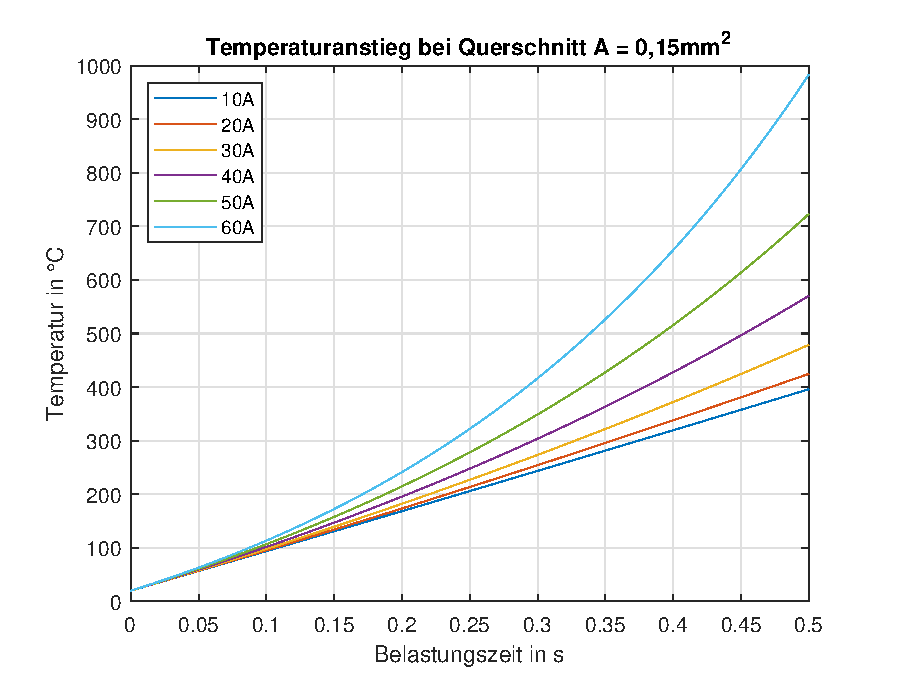
\includegraphics[width=247pt]{./Bilder/temp.eps}}
\subfigure{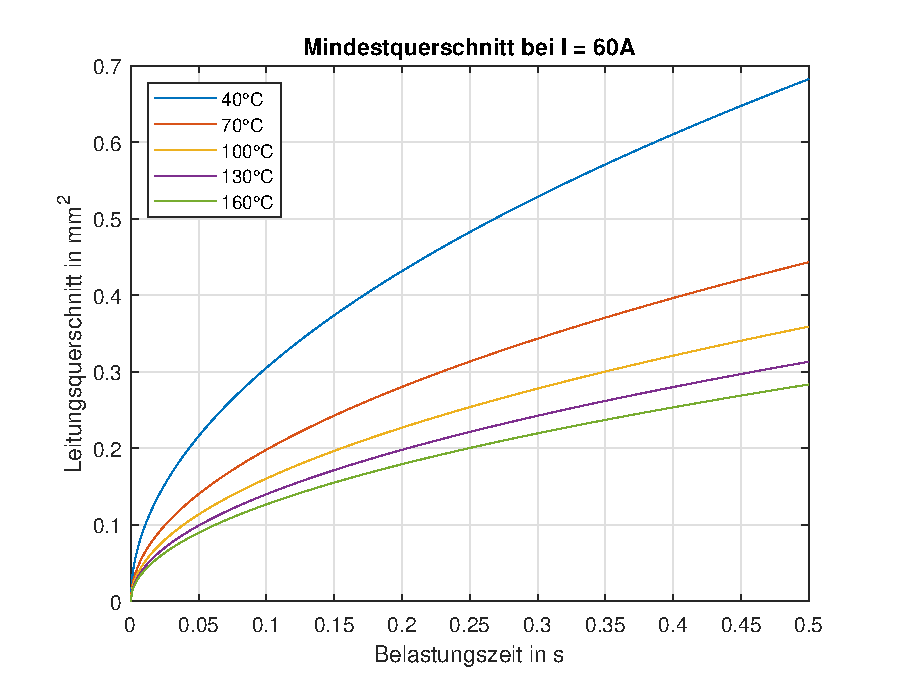
\includegraphics[width=247pt]{./Bilder/quer.eps}}
\caption{Dimensionierungsauswirkungen Temperatur und Leitungsquerschnitt}%
\label{fig:dimensionierung}%
\end{figure}\\
In \autoref{fig:dimensionierung} ist in der linken Abbildung der Temperaturanstieg über die Belastungsdauer bei verschiedenem Stromfluss und konstantem Querschnitt zu sehen. Es lässt sich erkennen, dass die Temperatur stärker über die Zeit ansteigt, je höher der Stromfluss über die Leiterbahn ist. Weiterhin ist der Steigungsverlauf exponentiell. In der rechten Abbildung ist der minimale Leitungsquerschnitt über die Belastungszeit bei konstantem Strom und verschiedenen zulässigen Maximaltemperaturen zu sehen. Der Verlauf des Leitungsquerschnittanstiegs ist logarithmisch und bei niedrigeren zulässigen Leitungsmaximaltemperaturen steigt der benötigte minimale Leitungsquerschnitt. 
\subsection{Anwendung auf realer Platine}
Die Kenndaten für die minimale Dimensionierung und die Kennwerte des Platinenmaterials sind in \autoref{tab:kennPl} beschrieben. Als Maximaltemperatur wurde dabei der Wert \SI{80}{^{\circ}C} gewählt. Der FR4-Kern der Platine ist nach Angaben des Herstellers für eine Temperatur bis zu \SI{135}{^\circ C} ausgelegt. Die lineare Temperaturabhängigkeit des Kupfers gilt annähernd im Bereich von -50...\SI{150}{^{\circ}C}\cite[S. 9]{Stiny2015}. Weiterhin ist die Anforderung an die Bauelemente, dass sie einen Temperaturbereich von mindestens -40...\SI{105}{^{\circ}C} abdecken. Um sich innerhalb dieser Bereiche zu bewegen und bei Temperaturausschlägen einen Sicherheitsfaktor zu berücksichtigen, sind die Leiterbahnen für die Maximaltemperatur von \SI{80}{^{\circ}C} auszulegen. Nach \autoref{tab:kennPl} ist für eine Kupferschichtdicke von \SI{70}{\mu m} eine Leiterbahnbreite von mindestens \SI{2,61}{mm} zu wählen. Beim Platinendesign ist diese aus Sicherheitsgründen zu \SI{3}{mm} gewählt, was einem maximalem Stromfluss von etwa \SI{69,1}{A} entspricht. Die Dimensionierung betrifft die Spannungsversorgungsleiterbahnen von der Batterie zu den Halbbrücken und die Leiterbahnen von den Halbbrücken zum Aktorklemmblock. Die restlichen Leiterbahnen auf der Platine sind für Dauerlast nach IPC 2221 auszulegen. Im Anhang findet sich ein Tabellenauszug nach IPC 2221 für die Strombelastbarkeit und eine Tabelle der Leistungsdaten der Platinenelemente, nach der die Leiterbahnen dimensioniert sind.
\begin{table}[H]%
\centering
\begin{tabular}{l l l l}
Kenngröße & Zeichen & Wert & Einheit\\ \hline
Temperaturkoeffizient Cu (20°C) & $\alpha_{20}$ & $3,93\cdot 10^{-3}$ &\SI{}{K^{-1}}\\
Spez. Widerstand Cu & $\rho$ & $1,721\cdot10^{-2}$ & \SI{}{\frac{\Omega\cdot mm^2}{m}}\\
Spez. Wärmekapazität Cu & c & 385 & \SI{}{\frac{J}{kg\cdot K}}\\
Dichte Cu & $\varrho$ & 8,92 & \SI{}{\frac{g}{cm^3}}\\
Referenztemperatur & $T_{20}$ & 20 &\SI{}{^\circ C}\\
Maximalstrom & $I_{max}$ & 60 & \SI{}{A}\\
Belastungsdauer & $t_i$ & 0,1 &\SI{}{s}\\
Maximaltemperatur & $T(t_i)$ & 80 & \SI{}{^\circ C}\\
Kupferschicht Dicke & d & $70\cdot 10^{-6}$ &\SI{}{m}\\
& & \\
resultierender Querschnitt & A & 0,1824 & \SI{}{mm^2}\\
resultierende Leiterbahnbreite & b & 2,6059 &\SI{}{mm}\\
\end{tabular}
\caption{Kenndaten Platine mit Kupferschicht}
\label{tab:kennPl}
\end{table}
\section{Routen der Platine}
Bei der letztendlichen Verlegung (\textit{routing}) der Leiterbahnen gibt es mehrere Aspekte zu beachten, die einerseits Einfluss auf die Elektromagnetische Verträglichkeit (\textit{EMV}), andererseits auch auf die Komplexität des Routingvorgangs haben.
\subsection{Design-Regeln und EMV}\label{sec:design}
Das Verlegen langer Leitungen sollte nach Möglichkeit vermieden werden um potentielle Störgrößen wie elektromagnetische Induktion und kapazitives Leitungsverhalten zu verringern \cite{haendschke}. Wie bereits in Abschnitt \autoref{sec:bau} erwähnt, sollten deshalb eine gewisse Lokalität der Bauteile eingehalten werden. Um die Leiterbahnen verlegen zu können sollten die Leiterplattenebenen (\textit{Layer}) abwechselnd verschiedene präferierte Verlegerichtungen aufweisen, sodass die Signale leicht an jeden Punkt der Platine verlegt werden können. In \autoref{fig:layer} ist schematisch der Aufbau einer zwei Layer Platine dargestellt. Im Falle einer gleichen Verlegerichtung kann es auftreten, dass sich die Signalleitungen auf keinem der vorhandenen Layer kreuzen können und somit unnötig lange Leitungen verlegt werden müssen \cite{haendschke}. Signale können zwischen den Platinen-Layern über Durchkontaktierungen (\textit{vias}) wechseln. Durchkontaktierungen sollten jedoch so selten wie möglich genutzt werden, da diese induktives Leitungsverhalten bewirken. In der Abbildung ist diese metallische Durchkontaktierung zwischen Layer 1 und Layer 2 exemplarisch dargestellt. Eine Signalleitung in Layer 1 kann, wenn sie mit der Metallfläche der Via verbunden ist, in Layer zwei weiter verlegt werden.
\begin{figure}[H]%
\centering
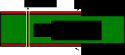
\includegraphics[width=300pt]{./Bilder/layer}%
\caption{Darstellung einer zwei Layer Platine inklusive Via}%
\label{fig:layer}%
\end{figure}
Prinzipiell können Platinen mit deutlich mehr Layer-Ebenen entworfen werden, zwei Layer Platinen werden jedoch bei industriellen Endprodukten aufgrund ihrer geringen Kosten präferiert \cite[S.13]{emcdes}. Im endgültigen Platinendesign wurde sich deshalb auch für eine zwei Layer Platine entschieden. Beim Verlegen der Leiterbahnen sollte weiterhin darauf geachtet werden, dass möglichst keine Winkel über \SI{45}{Grad} auftreten, da diese unerwünschte Reflektionen hervorrufen können \cite[S.17]{emcdes}. Bei wichtigen Signalleitungen sollte darauf geachtet werden, dass der Abstand zu anderen Leitungen größtmöglich ist, um eine Rückwirkung der Leiter aufeinander zu minimieren. Zur Verbesserung der Schirmung der Signalleitungen gegeneinander wird häufig eine GND-Leitung zwischen den Signalleitungen verlegt, welche die Rückwirkung verringert \cite[S.45]{Franz2012}.
Wenn diese Grundregeln der Leiterbahnplanung bekannt sind, gibt es nach \cite[S.12]{emcdes} drei Schritte, die zu einer fertigen Platine führen:
\begin{itemize}
	\item Komponentenauswahl und Platzierung (siehe \autoref{ch:komp} und \autoref{sec:bau})
	\item Entwurf des Versorgung- und Entkopplungskonzepts
	\item Verlegen der Signalleitungen
\end{itemize}
Nachdem in \autoref{sec:bau} die Bauteilplatzierung erläutert wurde, ist in \autoref{fig:logb} der erste Entwurf der Logikebene der Platine mit Versorgungskonzept und verschalteten Abblockkondensatoren zu sehen. Die Versorgungsleitungen werden dabei vor den Signalleitungen verlegt, da diese je nach Leistungsführung in ihrer Breite angepasst werden müssen. Die Logikebene beschränkt sich in dem Entwurf auf den STM32 und einen CAN-Transciever mit Pin-Ausgängen zur Ansteuerung der H-Brücke. Im dritten Schritt werden dann die Signalleitungen verlegt. Die Abbildung ist nur exemplarisch erstellt und wurde nie in Auftrag gegeben. Sie soll lediglich eine Nachvollziehbarkeit der Herangehensweise bewirken.
\begin{figure}[H]%
\centering
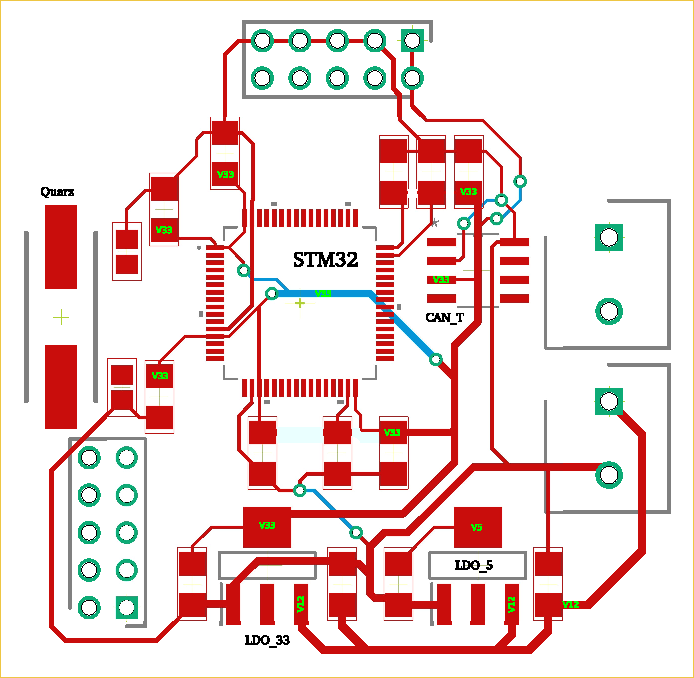
\includegraphics[width=250pt]{./Bilder/logb}%
\caption{Logikboard zur Endplatine inklusive Versorgungsleitungen}%
\label{fig:logb}%
\end{figure}
Üblicherweise werden zur Verbesserung der EMV nach dem Verlegen der Leiterbahnen die freien Platinenflächen zur Abschirmung auf GND Niveau gesetzt, welche als Teilmassenflächen bezeichnet werden. In der einschlägigen Literatur wird darauf hingewiesen, dass diese mit Vorsicht behandelt werden müssen, da Resonanz- und Antenneneffekte auftreten können. Um diesen Effekten vorzubeugen müssen die Masseflächen so gut wie möglich miteinander verbunden werden, sodass diese bei richtigem Anschluss die Schirmungsfunktion übernehmen \cite[S.166]{Franz2012}. Bei einem Layout mit 4 oder mehr Layern wird empfohlen vollständige GND-Layer und Versorgungslayer einzuführen, sodass eine optimale Abschirmung erfolgen kann \cite[S.172]{Franz2012}. Ein weiterer Effekt der im Bezug auf GND-Flächen betrachtet werden sollte ist das so genannte GND-Bouncing. Dieser Effekt tritt auf, wenn man keine gute Verbindung zwischen den GND-Flächen hat und somit unterschiedliche GND-Potentiale entstehen. Verstärkt wird dieser Effekt von Switching-ICs, also aktiven Bauteilen mit Schaltcharakteristiken, welche teilweise beim gleichzeitigen Umschalten von 1 nach 0 einen Zeitpunkt aufweisen, zu dem VCC und GND kurzgeschlossen sind und sich somit das GND Potential kurz anhebt \cite[S.1]{gndbnc}. Aufgrund dieses Effektes sollte die GND-Fläche so gut wie möglich verbunden sein um das GND Potential gleichmäßig zu halten. Problematisch ist dabei auch nicht zwingend wenn es kein geschlossenes GND-Layer gibt, solange die GND-Verbindungen der Ebenen sich außreichend überlappen und über Durchkontaktierungen gut verbunden sind \cite[S.172]{Franz2012}. Zur Abschirmung der aktiven Bauelemente gegen Welligkeiten der Spannungsversorgung werden wie in \autoref{ch:komp} erwähnt Abblockkondensatoren verwendet. Dabei sollten möglichst SMD Bauteile genutzt werden um entstehende parasitäre Induktivitäten zu verringern \cite[S.34]{emcdes}. Als Abschirmung gegen von außen autretende elektromagnetische Felder sei die Schirmwirkung von Kühlkörpern oder Gehäuseteilen aus Metall hervorgehoben \cite[S.22]{Franz2012}.

\subsection{Leiterbahnverlegung des Entwicklungsboards}
Die Verlegung der Leiterbahnen auf dem endgültigen Entwicklungsboard geschieht nach den zuvor definierten Designregeln, wobei aufgrund des geringen Platzes häufig Kompromisse eingegangen werden müssen. Das Entwicklungsboard weist 2 Layer auf, welche der Anordnung aus \autoref{fig:layer} entsprechen und im Folgenden über die Bezeichnung Top-Layer (obere Leiterebene) und Bottom-Layer (untere Leiterebene) gekennzeichnet werden. Grundanforderungen an die Platine ist die Positionierung der GND-Löcher, durch welche die Platine mittels Schrauben über das Aktorgehäuse mit GND verbunden ist. In \autoref{fig:top} und \autoref{fig:bot} ist das fertige Top-und Bottom-Layer der Platine zu sehen. Problematisch für das Einhalten der Designregeln ist hauptsächlich die Platzierung der Halbbrücken und der mittleren Schraubenlöcher, welche den Platz für die Signalleitungen von dem Mikrocontroller in Richtung Platinenstecker stark begrenzen. Die präferierte Verlegerichtung auf dem Top-Layer ist vertikal gewählt um die jeweiligen ICs über kurze Wege ohne große Leitungsverluste erreichen zu können. Dabei liegen CAN-Transciever und Leitungsverstärker oberhalb und der externe Schwingquarz unterhalb des Mikrocontrollers, was optimal für die präferierte Leitungsrichtung ist. Problematisch ist die Leitungsverlegung in Richtung der Halbbrücken und des Steckers, da der Spalt zwischen Schraubloch und Halbbrücke in der oberen Platinenhälfte durch die Versorgungsspannung belegt ist. 
\begin{figure}[H]%
\centering
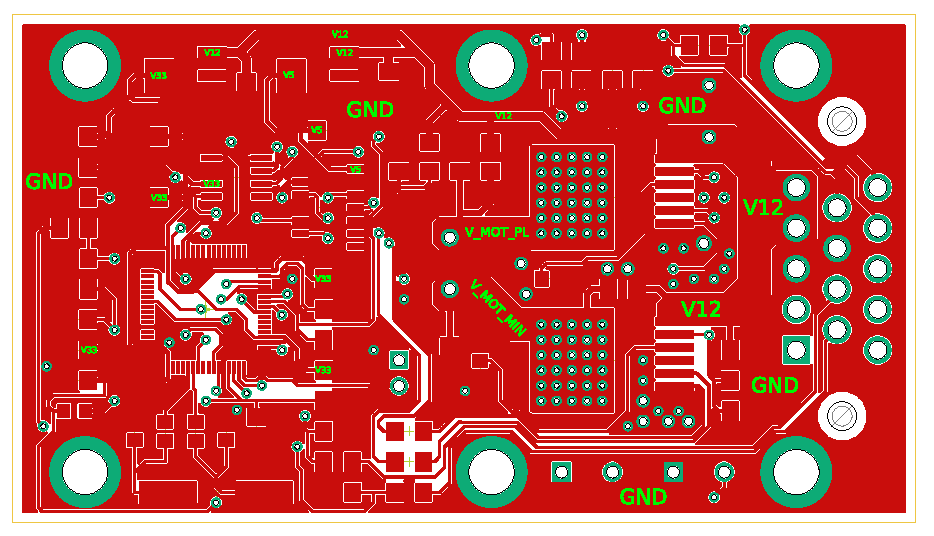
\includegraphics[width=400pt]{./Bilder/top2}%
\caption{Darstellung des Top-Layers}%
\label{fig:top}%
\end{figure}
Die präferierte Verlegerichtung des Bottom-Layers ist horizontal ausgerichtet, sodass diese Leiterebene hauptsächlich zum Erreichen der Halbbrücken und des Steckers genutzt wird. Bei Betrachtung von \autoref{fig:bot} fällt jedoch auf, dass der Platz für die Leitungen sehr begrenzt ist und somit ein Teil der horizontalen Leiterbahnen auf das Top-Layer verlegt werden musste. Eine weitere wichtige Aufgabe beim Verlegen der Leiterbahnen ist die Reduktion elektromagnetischer Rückwirkung, wobei sich an die Methoden aus \autoref{sec:design} gehalten wird. Potentielle Gefahrenquelle der Rückstrahlung sind die Halbbrücken, da diese beim Schalten mit PWM-Signal Stromimpulse in hohen Frequenzen durchschalten können. Wichtige Signalleitungen wie die der Sensorik sind also möglichst weit von den Flächen mit der Bezeichnung V\_MOT\_PL und V\_MOT\_MIN (Halbbrücken Ausgänge) zu verlegen. Aufgrund des Platzmangels lassen sich die Signalleitungen der Sensorik nicht vollständig aus dem Einflussgebiet der Halbbrücken entfernen, sind jedoch von diesen so weit wie möglich entfernt verlegt. Bei genauerer Betrachtung der Layer fällt auf, dass jedoch trotzdem Signalleitungen nahe des Einflussgebietes der Halbbrücken verlaufen. Diese Leiterbahnen sind hauptsächlich die Leiterbahnen der SWD-Verbindung, also der Programmierschnittstelle der Platine. Daher stellt dies kein Problem dar, da die Platine nicht im laufenden Aktorbetrieb programmiert wird und somit die Lokalität im Einflussgebiet der Halbbrücken kein Hindernis darstellt. Die Leitungen zur Ansteuerung der Halbbrücken HB1\_IN und HB2\_IN sollten ebenfalls nicht im direkten Einflussgebiet liegen, damit die Halbbrücken vom Mikrocontroller noch problemlos angesteuert werden können. Als Konzept zur Abschirmung elektromagnetischer Rückwirkung wurde bereits der Einsatz von Abblockkondensatoren erwähnt, der eine wesentliche Rolle spielt. Neben diesen sind die freien Boardflächen auf beiden Layern auf GND-Potential gesetzt um damit ebenfalls Schirmungseffekte erzielen zu können. Diese sind zwar auf beiden Layern nicht optimal zusammenhängend, es wurde aber darauf geachtet über Durchkontaktierungen eine stabile gemeinsame GND-Fläche zu erhalten, welche gegen GND-Bouncing geschützt ist. Die GND-Flächen werden ebenfalls über die Aluminiumplatte und den Aktor auf ein gleichmäßiges Potential gezogen. Neben den EMV-Maßnahmen sollte auch die Wärmeentwicklung der Bauteile berücksichtigt werden. Aufgrund des hohen Stromflusses stellen die Halbbrücken besondere Anforderungen an die Kühlung. Insbesondere in Transistorschaltvorgängen innerhalb der Halbbrücke während denen ein Teil der Versorgungsspannung an den Transistoren abfällt und somit nach $P = U\cdot I$ erhöhte Wärmeenergie entsteht. Um die Halbbrücken unter ihrer kritischen Temperatur halten zu können, muss die entstehende Wärme abgeführt werden. Dies kann beispielsweise durch Durchkontaktierungen (\textit{Thermische Vias}) unter den kritischen Bauteilen erreicht werden. Über die Thermischen Vias vergrößert sich die zusammenhängende Metallfläche auf der sich die Wäre ausbreiten kann in das Bottom-Layer, und kann somit gut über den anliegenden Aluminium-Körper abgeführt werden.
\begin{figure}[H]%
\centering
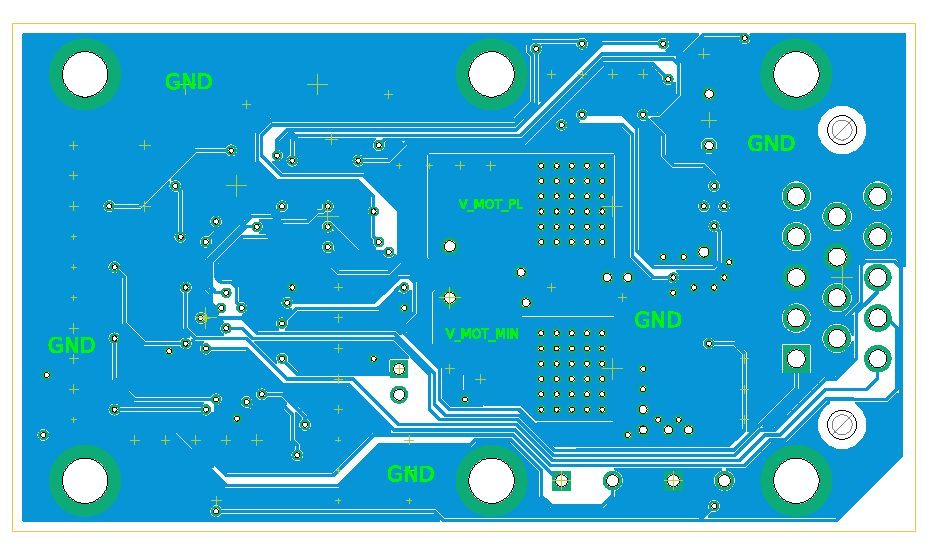
\includegraphics[width=400pt]{./Bilder/bottom2}%
\caption{Darstellung des Bottom-Layers}%
\label{fig:bot}%
\end{figure}

\newpage
\section{Fertigung}
In \autoref{fig:platop} und \autoref{fig:plabot} ist die Platine nach dem Fertigungsprozess zu sehen. Als Kenndaten für die Fertigung wurde eine Leiterbahndicke von \SI{70}{\mu m} festgelegt. Als Kern wird ein FR4 Verbundwerkstoff mit einer Dicke von \SI{1,5}{mm} verwendet. Gut zu sehen sind auf den fertigen Leiterplatten auch die thermischen Vias, welche in das Lötpad von HB\_1 und HB\_2 eingelassen sind.
\begin{figure}[H]%
\centering
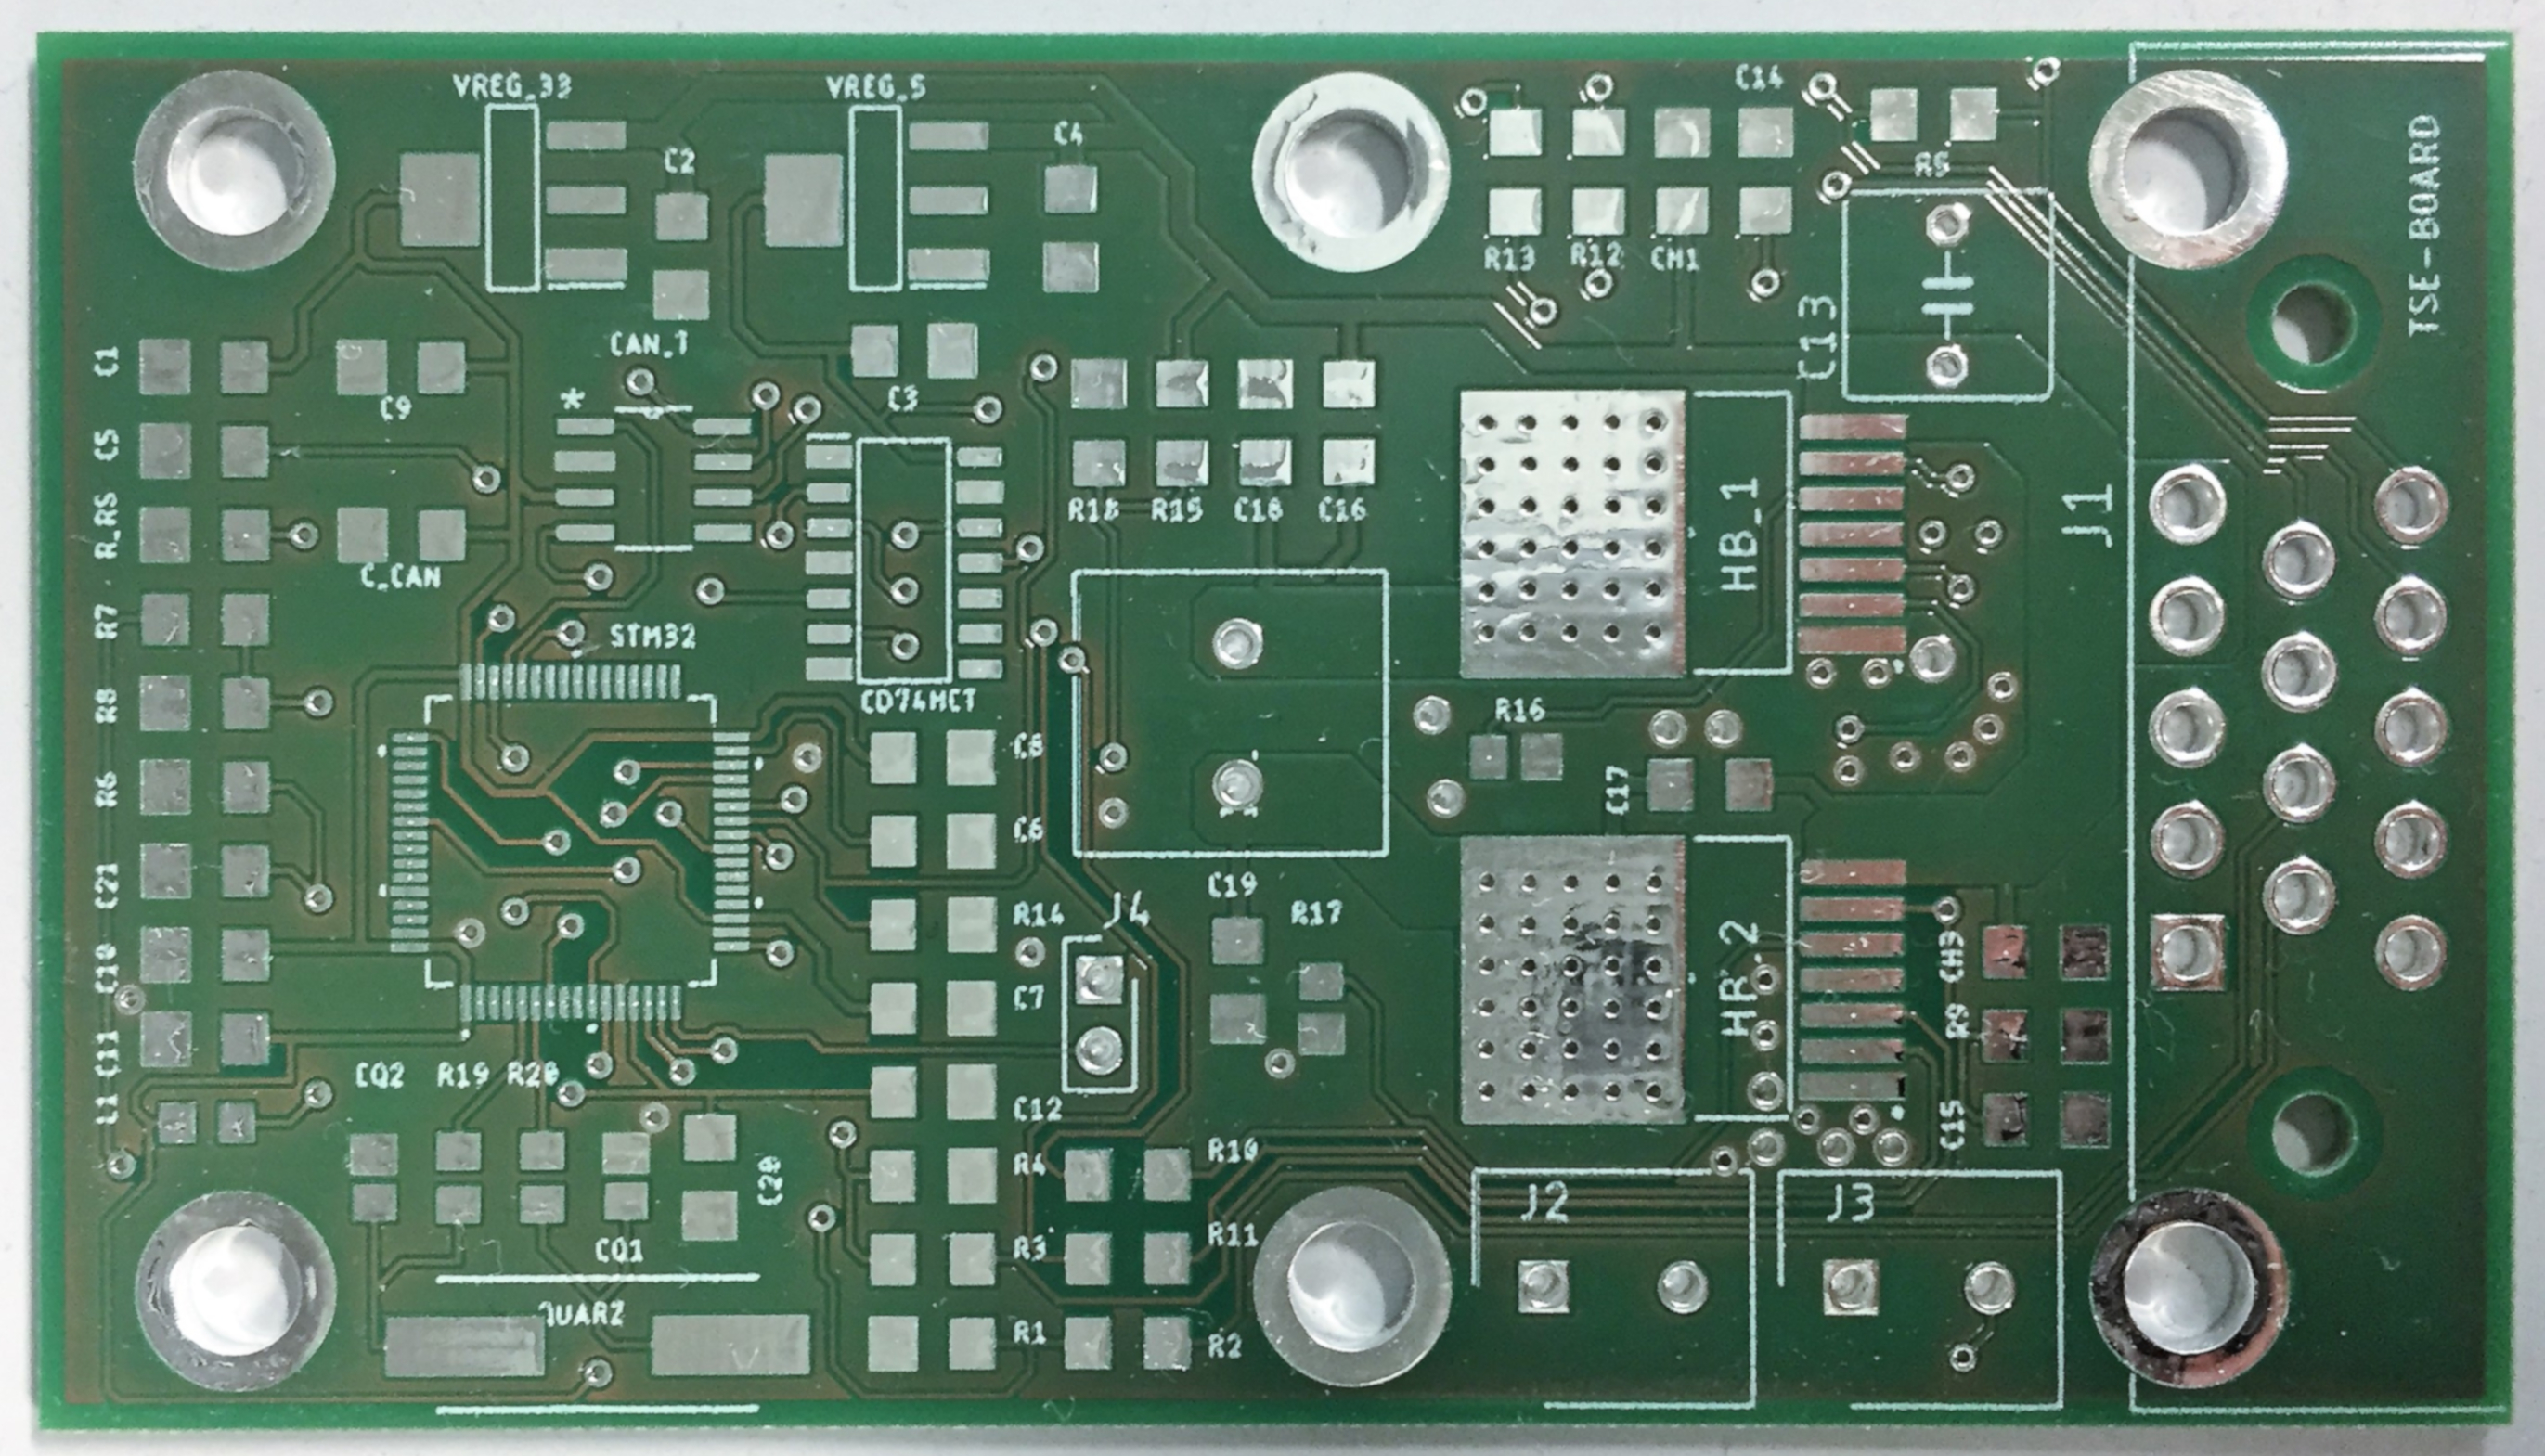
\includegraphics[width=400pt]{./Bilder/pla_top2}%
\caption{Top-Layer nach dem Fertigungsprozess}%
\label{fig:platop}%
\end{figure}
\begin{figure}[H]%
\centering
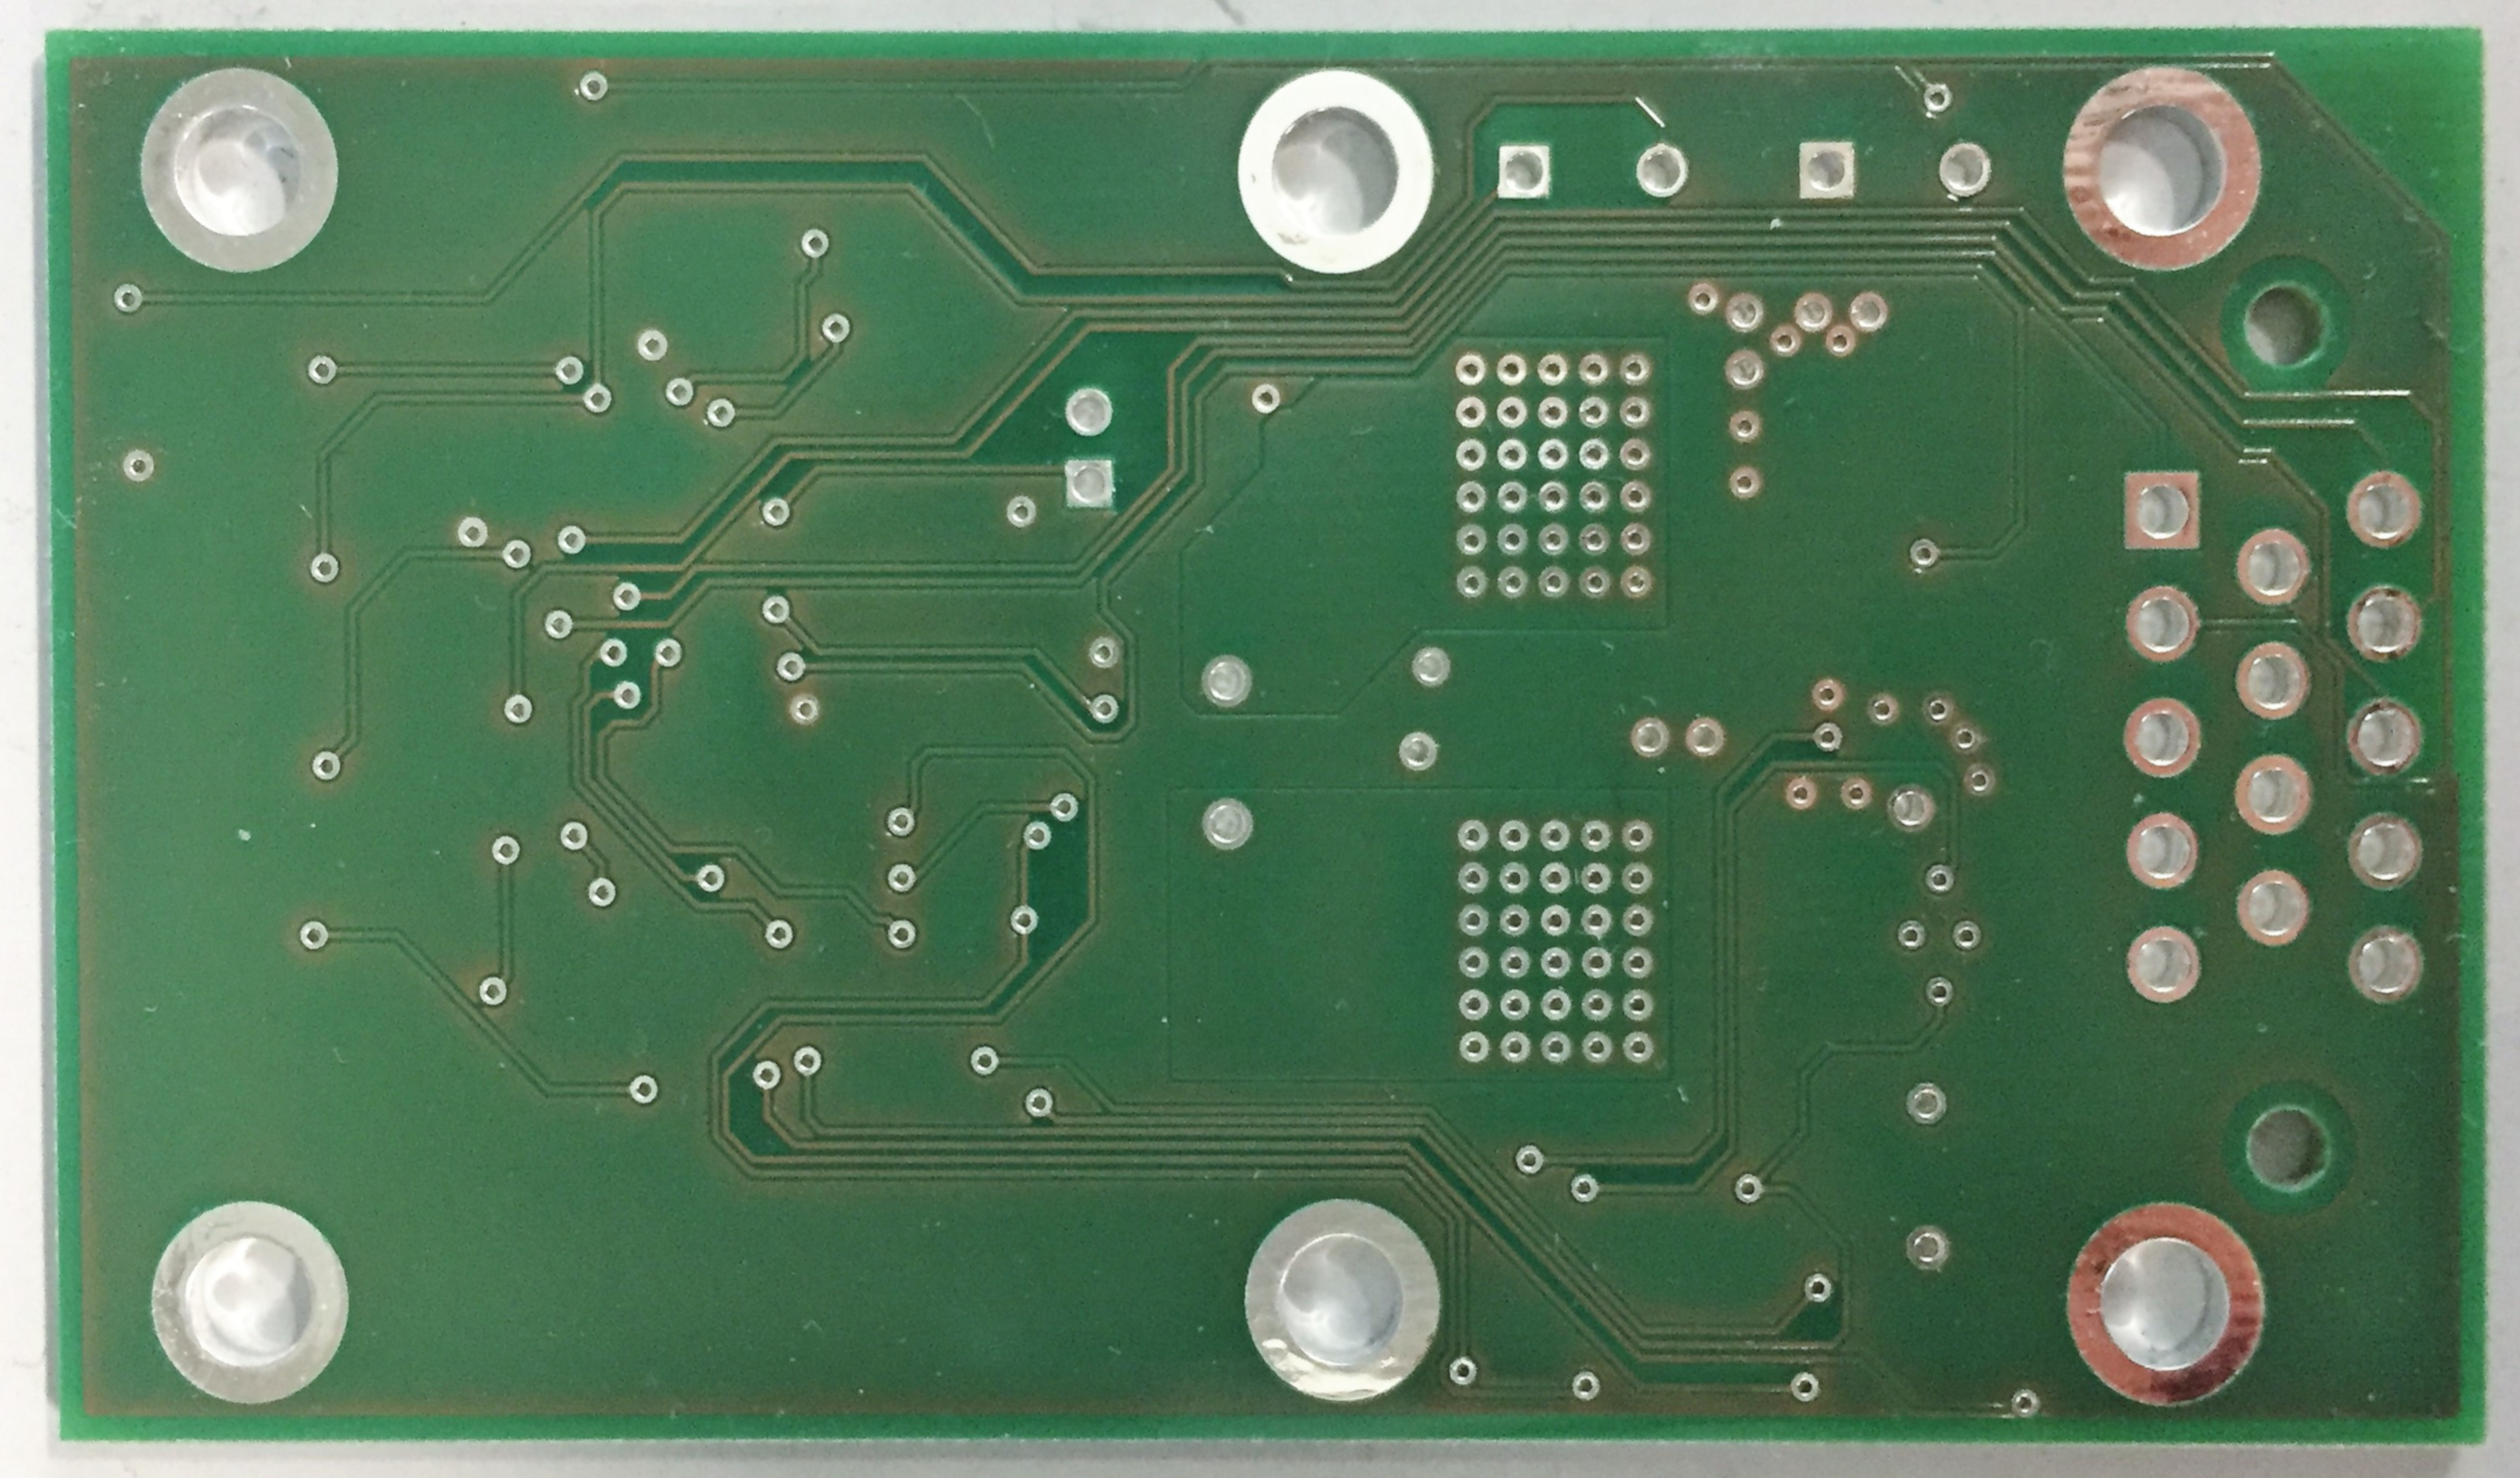
\includegraphics[width=400pt]{./Bilder/pla_bot2}%
\caption{Bottom-Layer nach dem Fertigungsprozess}%
\label{fig:plabot}%
\end{figure}